\documentclass[twocolumn, a4paper]{article}

\usepackage[T1]{fontenc}
\usepackage[utf8]{inputenc}
\DeclareUnicodeCharacter{2212}{-}
\usepackage[italian]{babel}

\usepackage{physics}

%%%%%%%%%%%%%%%%
%%% BELLURIE %%%
%%%%%%%%%%%%%%%%

%%%%%%%%%%%%
%%% font %%%
%%%%%%%%%%%%
\usepackage{libertinus}
\usepackage{libertinust1math} %AMS caricato in automatico
\newcommand*\diff{\mathop{}\!\mathrm{d}}

\usepackage{tabularx}
\usepackage{eurosym}
\usepackage{multirow}
\usepackage{microtype}

%%%%%%%%%%%%%%%%%%%%
%%% frontespizio %%%
%%%%%%%%%%%%%%%%%%%%
\usepackage{titling}

%titolo
\pretitle{\begin{center}\scshape\sffamily\LARGE}
\posttitle{\par\end{center}}
%autore
\preauthor{\begin{center}\large\scshape\sffamily\begin{tabular}[t]{c}}
\postauthor{\end{tabular}\par\end{center}}
%data
\predate{\begin{center}\large\sffamily}
\postdate{\par\end{center}}

%%%%%%%%%%%%%%%%
%%% sommario %%%
%%%%%%%%%%%%%%%%
\usepackage{abstract}
\renewcommand{\abstractnamefont}{\sffamily\large\scshape}
\renewcommand{\abstracttextfont}{\normalsize}
\setlength{\absleftindent}{6em}
\setlength{\absrightindent}{6em}

%%%%%%%%%%%%%%%%%%%%%%%%%%
%%% titoli e titoletti %%%
%%%%%%%%%%%%%%%%%%%%%%%%%%
\usepackage[sf, sc, medium, center, pagestyles]{titlesec}
\renewpagestyle{plain}[\scshape\sffamily]{
	\sethead{Proposta progetto \emph{Fly your experiment}}{}{SpaceLab, UniPi}
	\setfoot{}{\thepage}{}
}

\pagestyle{plain}

%%%%%%%%%%%%%
%%% ALTRO %%%
%%%%%%%%%%%%%
%\usepackage{pgf}
%\usepackage{rotating}
\usepackage{enumitem}
\setlist{leftmargin=*}
\usepackage{caption, subcaption}
\captionsetup{labelfont={bf, sc}, textfont=sf}
%\captionsetup[sub]{skip=0.2em}
\usepackage{booktabs}

\usepackage{mhchem, natbib, graphicx}
\graphicspath{{immagini/}}
\usepackage{hyperref}

%%%%%%%%%%%%%%%%%%%%%%
%%% NUOVO AMBIENTE %%%
%%%%%%%%%%%%%%%%%%%%%%
\newenvironment{crewbio}[1]{\noindent\textbf{#1} ---}{\\}

%%%
%%%
%%%

\title{Misura del flusso di raggi cosmici e separazione delle componenti carica e neutra.}
\author{Adriano Del Vincio \and Viola Floris \and Daniele Passaro \and Domenico Riccardi \and Marco Riggirello
\and
Niccolò Torriti \and Antoine Venturini}
\date{7 Maggio 2021}

%%%%%%%%%%%%%%%%%%%%%%%%%%%
%%% CORPO DEL DOCUMENTO %%%
%%%%%%%%%%%%%%%%%%%%%%%%%%%

\begin{document}
\maketitle

\section{Introduzione}
I raggi cosmici (RC) sono particelle elementari e nuclei  provenienti dall'universo che bombardano costantemente l'atmosfera terrestre. I RC sono solitamente classificati in due categorie: i \emph{primari}, ovvero le particelle cosmiche che incidono direttamente nell'alta atmosfera, tipicamente composti da protoni, particelle alpha e in parte minore da nuclei leggeri; i \emph{secondari}, prodotti dagli sciami adronici ed elettromagnetici generati dalle interazioni dei primari con l'atmosfera, e tipicamente composti da muoni, mesoni, adroni leggeri e nuclei.
\begin{figure}[h!]
\centering
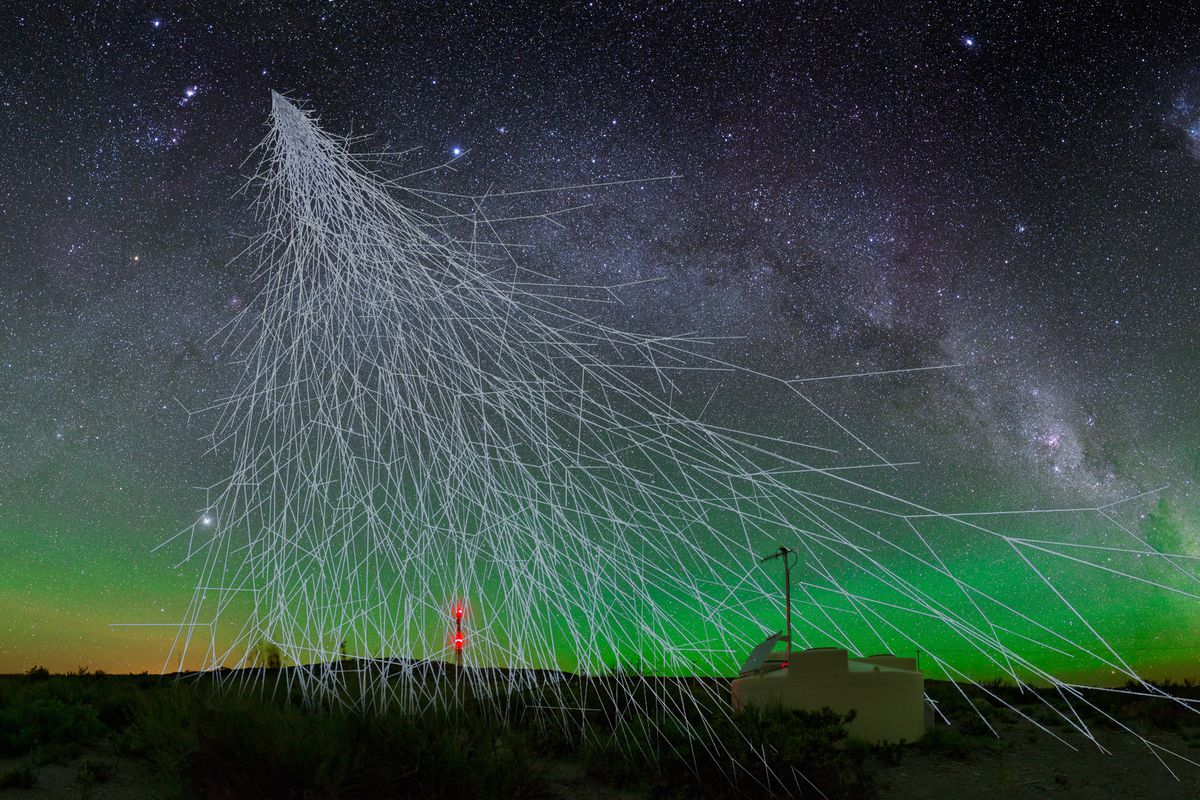
\includegraphics[width=0.9\linewidth]{pierre4HR.0.jpg}
\caption{Sciame prodotto da un raggio cosmico primario. \citep{immagine_cosmici}}
\end{figure}
 I RC sono noti fin dai primi decenni del '900 e la loro fisca è stata studiata approfonditamente nel corso degli anni. Ciononstante, alcuni aspetti non sono stati approfonditi, per cui risulta tutt'ora di grande interesse scientifico effettuare ricerca in questo campo. Le misure di interesse che vogliamo effettuare con il nostro esperimento sono: 
\begin{enumerate}
    \item \textbf{Misura di flusso verticale dei RC carichi in funzione dell'altitudine} - Il flusso verticale di raggi cosmici è atteso dipendere dalla quota: l'interazione adronica dei primari con l'atmosfera (Figura \ref{frammentazione primari}) dipende criticamente dalla densità del mezzo. Stimiamo che il massimo della produzione di secondari avvenga attorno ai 20km. Questa misura è di duplice interesse: correlazione con l'altitudine di formazione delle nuvole, rivelando un possibile ruolo dei RC nella loro formazione (esperimento CLOUD @CERN); stima dei danni da radiazione indotti sull'elettronica, importante per stimare i \textit{single event upset} nella strumentazione di missioni spaziali;
    \begin{figure}
        \centering
        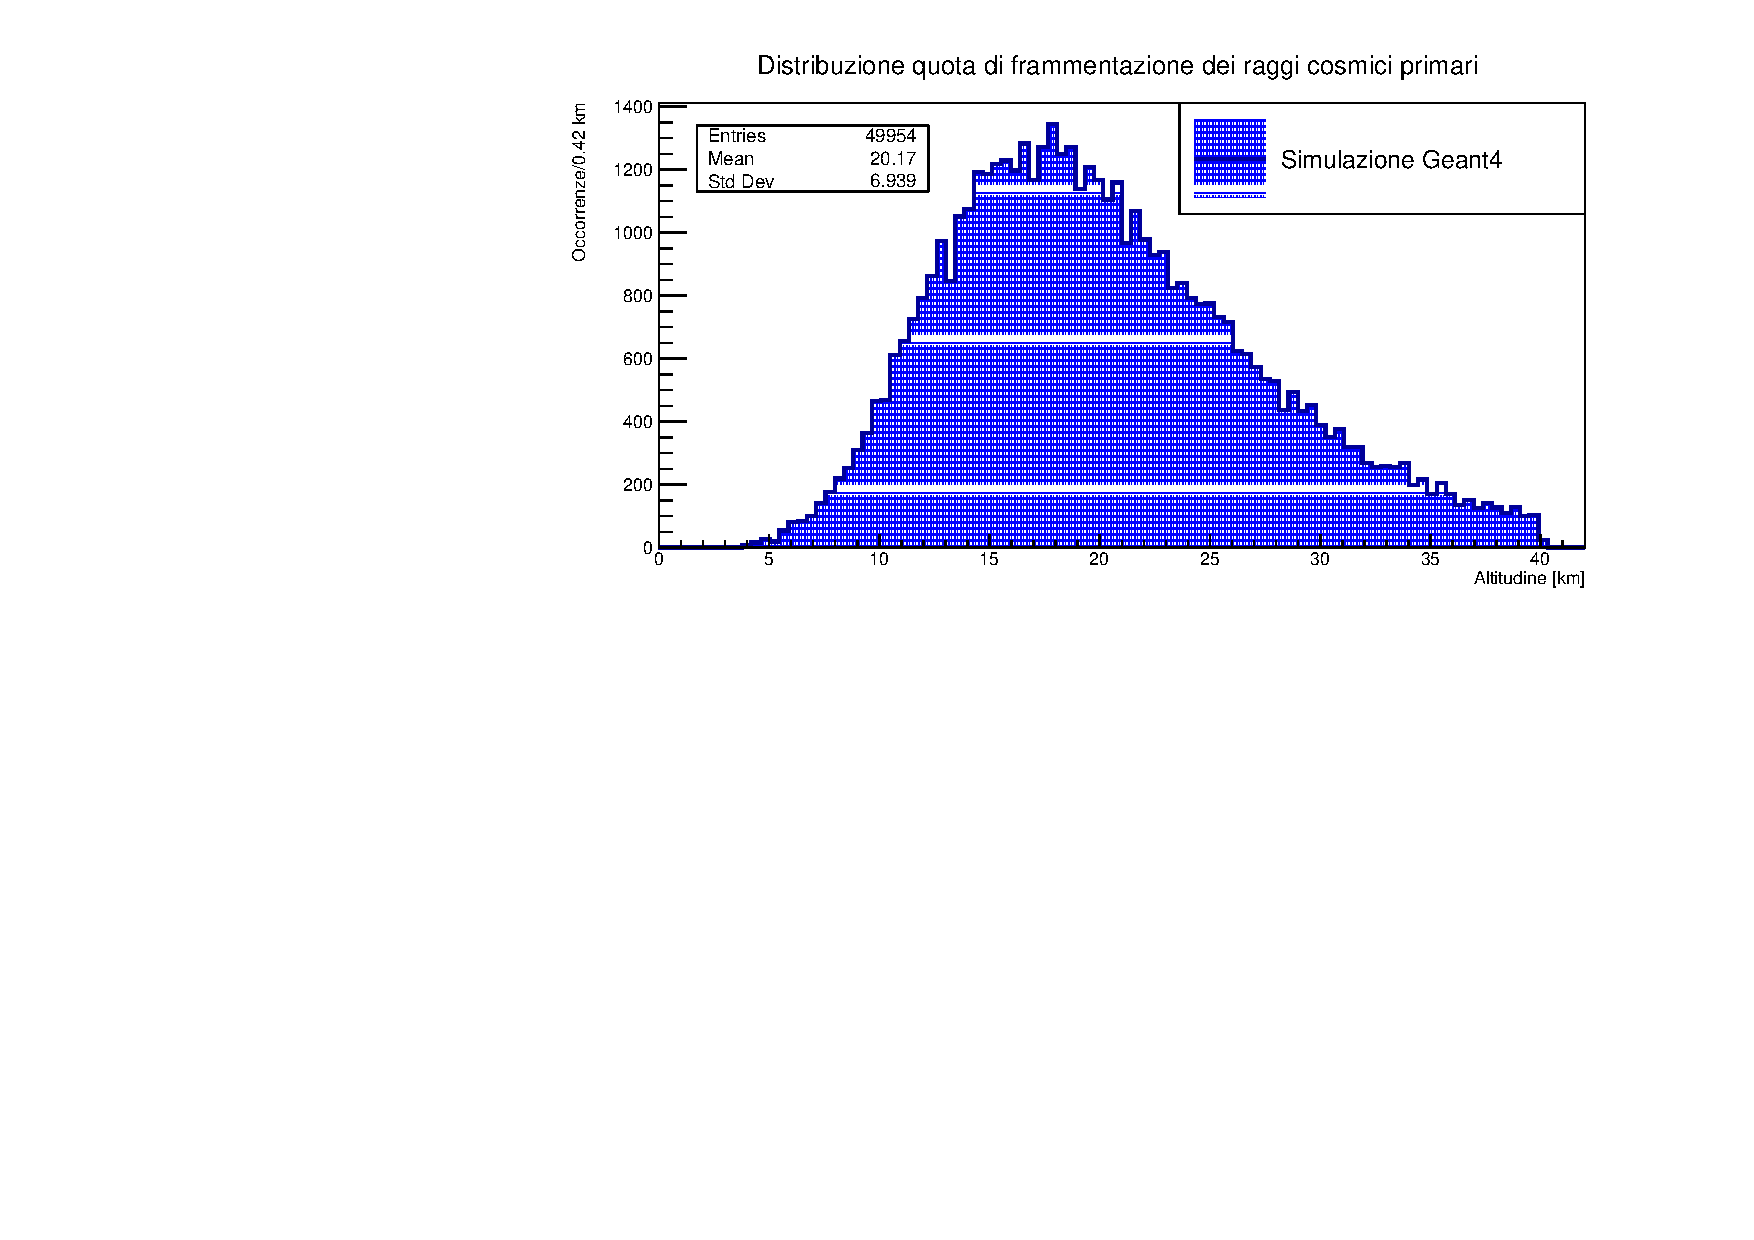
\includegraphics[width=0.9\linewidth]{Frammentazione_verticale.pdf}
        \caption{Simulazione GEANT4 della quota di frammentazione di un fascio di protoni energetici nell'atmosfera.}
        \label{frammentazione primari}
    \end{figure}
    
    \item \textbf{Misura di flusso orizzontale dei RC carichi in funzione dell'altitudine} - Ci si aspetta che la componente orizzontale dei RC sia fortemente soppressa, ma questo dipende dallo spessore trasverso di atmosfera attraversata, dunque dalla quota. Questa misura non è presente in letteratura e può apportare un contributo originale alla comprensione dei RC;
    \item \textbf{Misura del flusso di neutroni termici in funzione dell'altitudine} - I neutroni vengono prodotti in seguito a reazioni di spallazione nucleare tra la componente di raggi cosmici primari ed i nuclei di azoto e ossigeno. Lo spettro energetico risulta piccato per energie di $100\text{ KeV}$, come si osserva dalla Figura \ref{Neutroni}. Attraverso processi di scattering multiplo l'energia cinetica dei neutroni diminuisce, fino ad energie inferiori ad 1 $\text{eV}$. Neutroni con tale range di energie sono definiti termici. A queste energie diventano importanti fenomeni di assorbimento, in particolare si sottolinea il seguente:
\ce{n + ^{14}N -> ^{14}C + p}
, in cui da un nucleo di azoto si forma un particolare isotopo del carbonio. La reazione descritta regola la produzione e abbondanza relativa del carbonio-14 in natura. Dalla misura del flusso di neutroni termici possiamo ricavare il rate di produzione del $^{14}\text{C}$ in funzione della quota (Figura \ref{Carbonio}).
La misura è importante perché l'attività legata al carbonio-14 è uno dei metodi più diffusi di datazioni di reperti organici. 
\begin{figure}
    \centering
    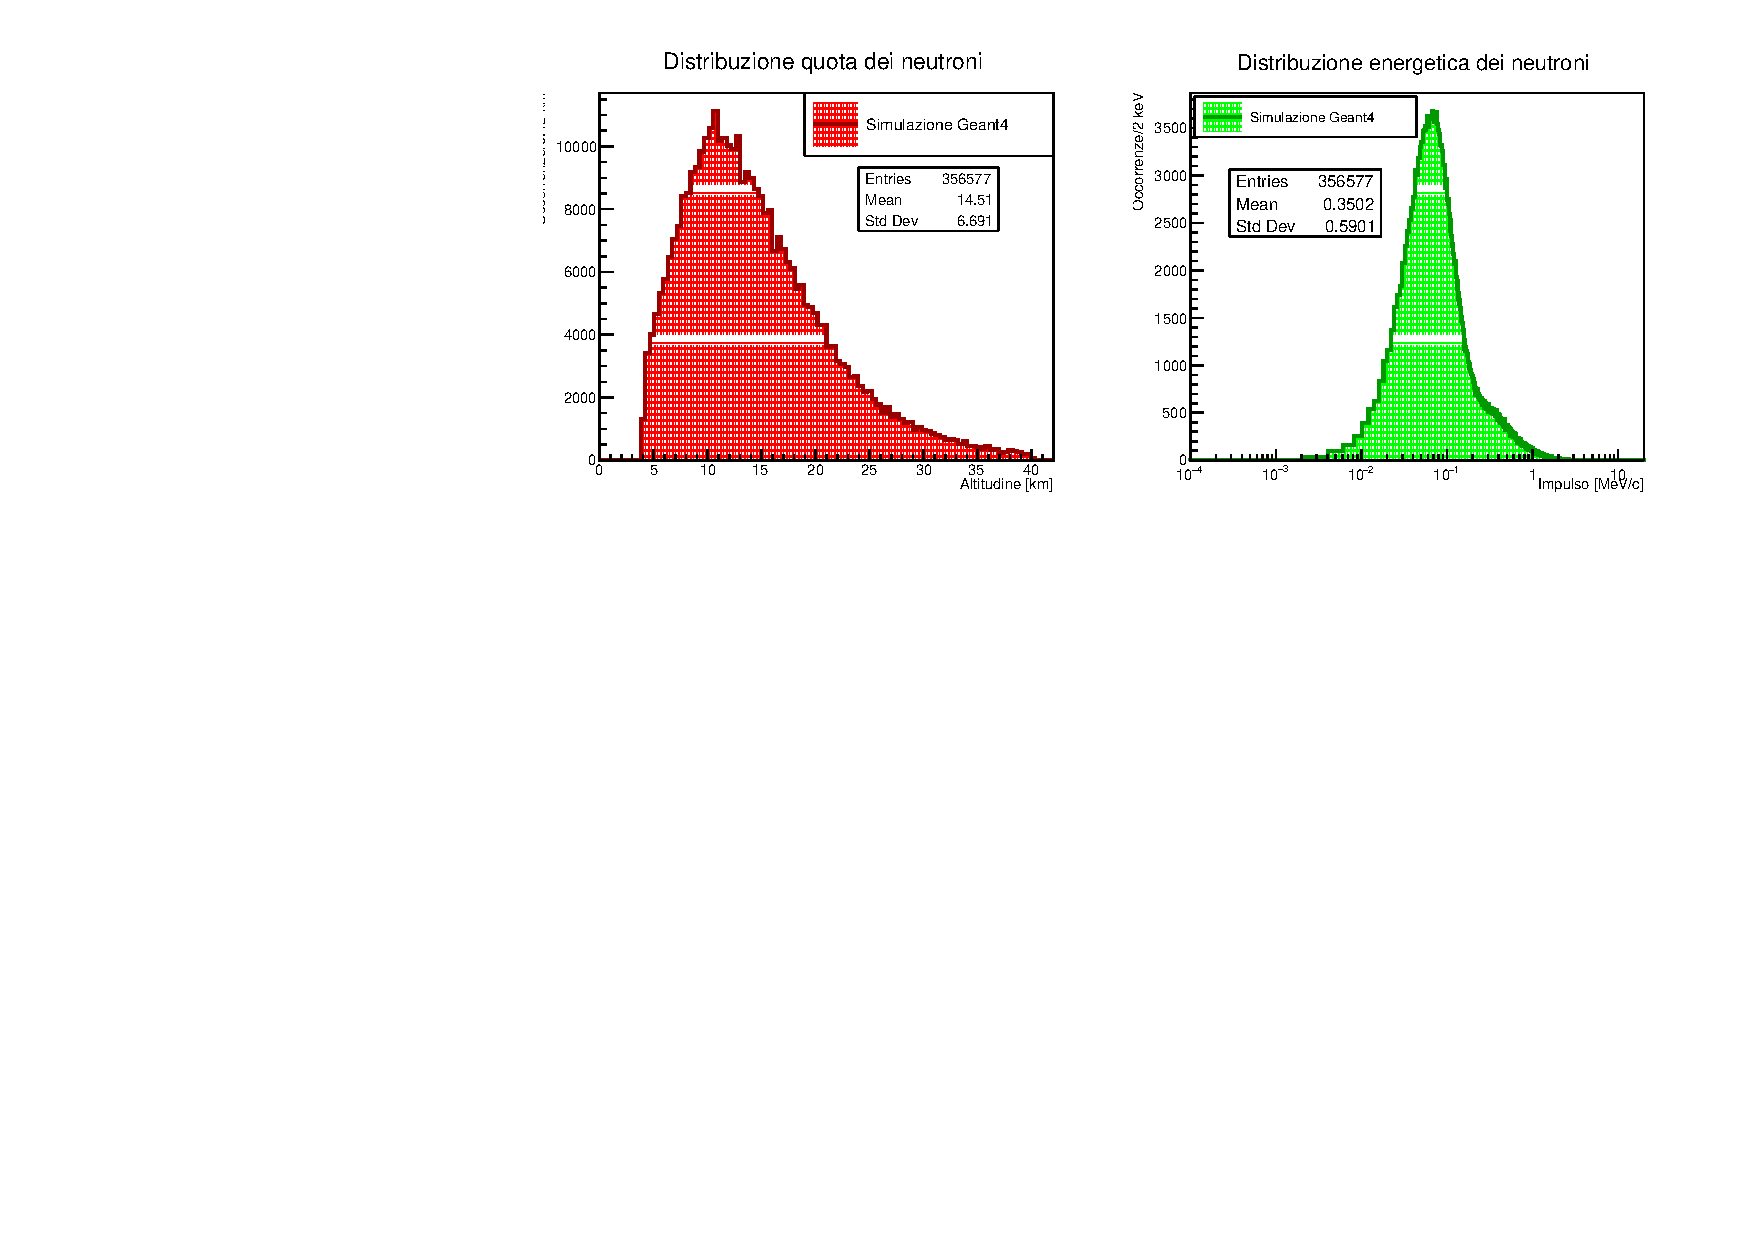
\includegraphics[width=.9\linewidth]{Neutroni.pdf}
    \caption{Simulzione GEANT4 della quota e spettro energetico iniziale dei neutroni prodotti. Si noti come la distribuzione in quota segue quella dei protoni primari (Fig. \ref{frammentazione primari}).}
    \label{Neutroni}
\end{figure}
\begin{figure}
    \centering
    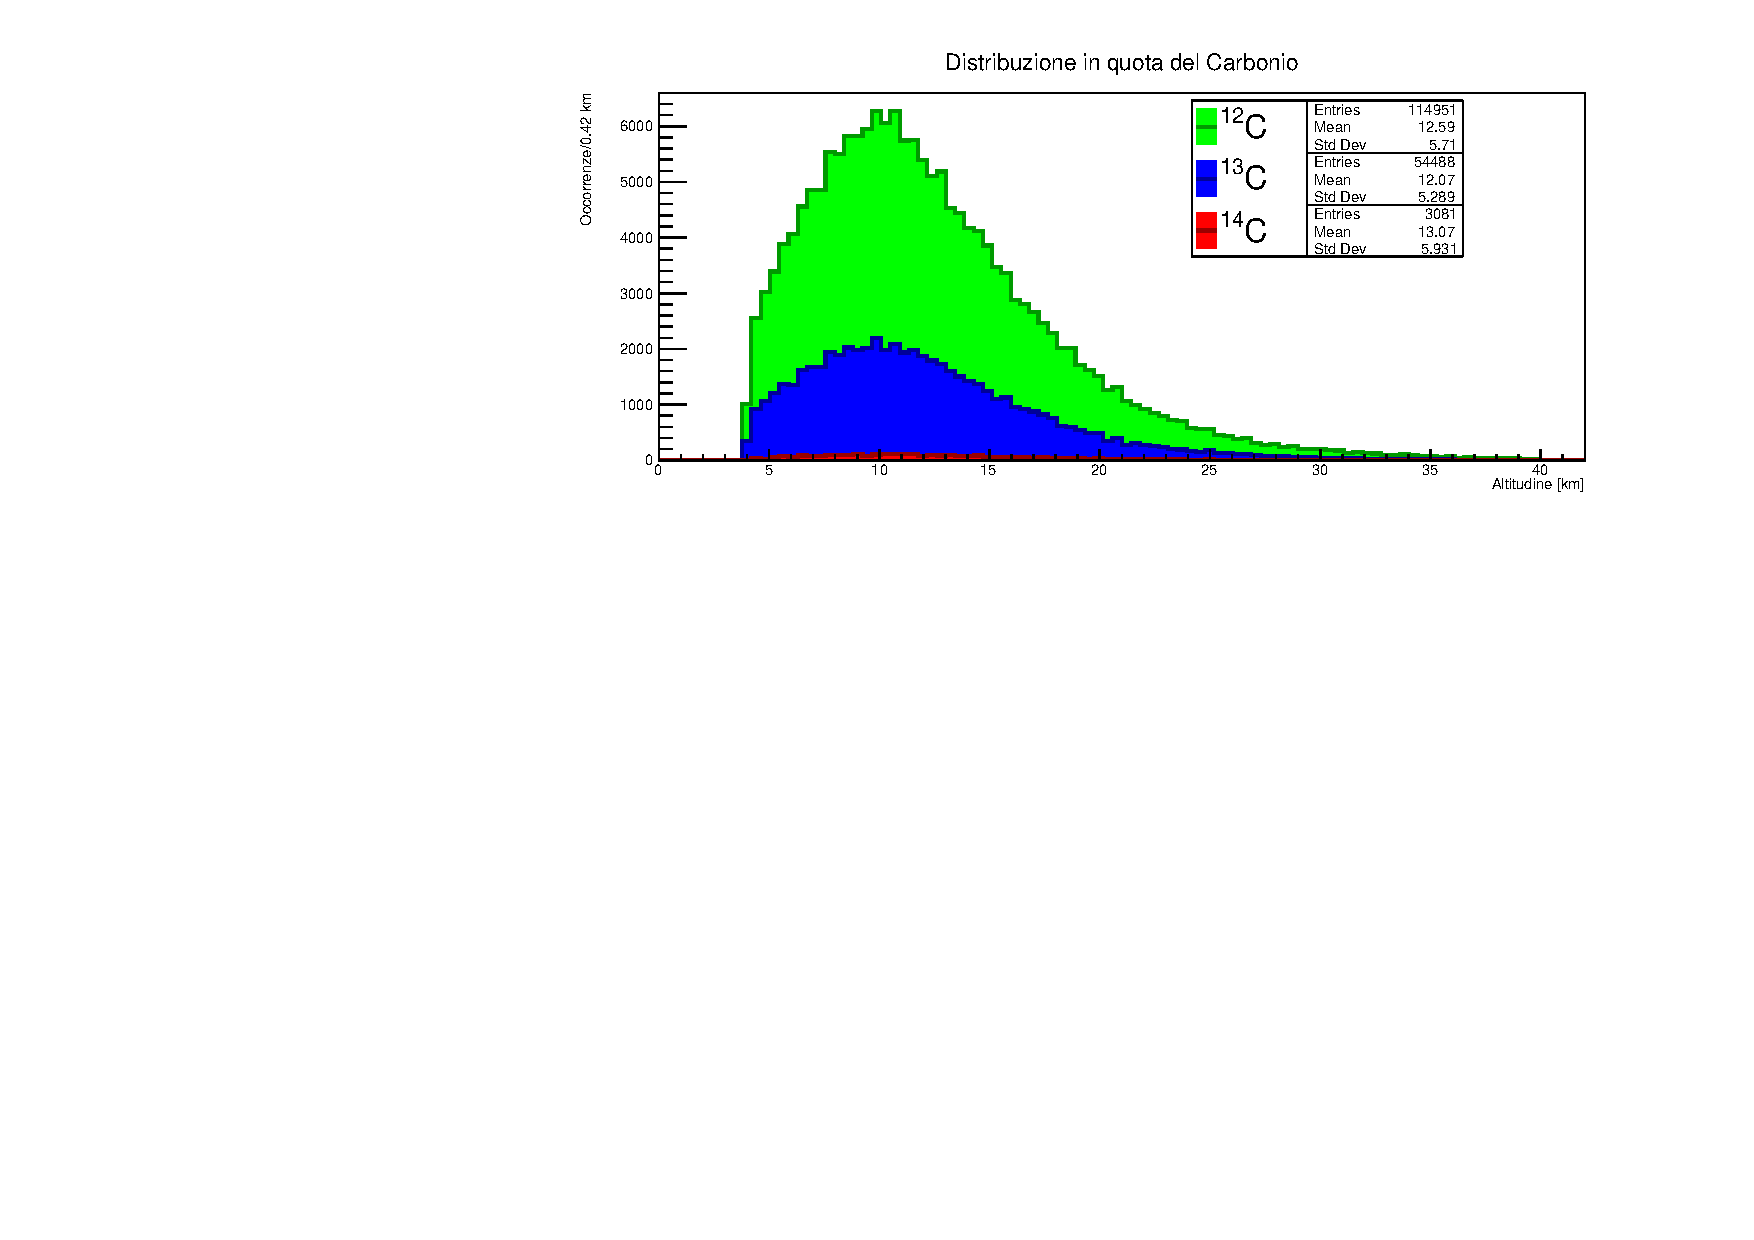
\includegraphics[width=.9\linewidth]{Carbonio_verticale.pdf}
    \caption{Simulazione GEANT4 della distribuzione in quota degli isotopi del C prodotti dai RC primari.}
    \label{Carbonio}
\end{figure}
    \item \textbf{Caratterizzazione del modulo rivelatore \emph{micromegas}} - Prodotto *** DA CHI *** appositamente per il nostro esperimento, ci proponiamo di caratterizzare  la risposta di questo rivelatore in ambienti estremi di temperatura e pressione. Questo lavoro potrebbe essere determinante nella futura applicazione della micromegas a      bordo di satelliti e missioni spaziali. ***** DA COMPLETARE CON ENA ********
\end{enumerate}
\bibliographystyle{plain}
\bibliography{references}

\section{Apparato Sperimentale}
Tutte le misure di flusso passano attraverso la conoscenza e lo studio dettagliato dell'efficienza dei singoli detector che costituiscono il nostro apparato. Tale studio sarà effettuato a terra presso i laboratori dell'INFN come operazione preliminare al volo, presumibilmente nelle settimane precedenti al lancio. 

La rivelazione della componente carica avviene attraverso due diversi apparati: due sistemi basati su scintillatori e una \emph{micromegas}. Entrambi i detector vengono sviluppati appositamente e gentilmente finanziati dall'INFN. 
\subsection{Scintillatore}
La prima classe di detector sfrutta il \emph{meccanismo di scintillazione} per rivelare le particelle cariche che attraversano un materiale plastico emettendo fotoni raccolti da due SiPM (Silicon PhotoMultiplier) incollati sulle pareti laterali. In particolare, i SiPM utilizzati saranno del tipo NUV (sensibili ultravioletto) della FBK\footnote{https://advansid.com/technology/silicon-photomultipliers}.
Questo sistema scintillatore--SiPM viene letto da un'elettronica di front-end essenzialmente suddivisa in due parti: PCB (che comprende l’amplificatore e il comparatore, oltre che il circuito di alimentazione dei SiPM) e CPU (XLR8 di Alorium con FPGA). Tale apparato è già stato assemblato come mostrato in Figura \ref{Telescopio}.
\begin{figure}
\centering
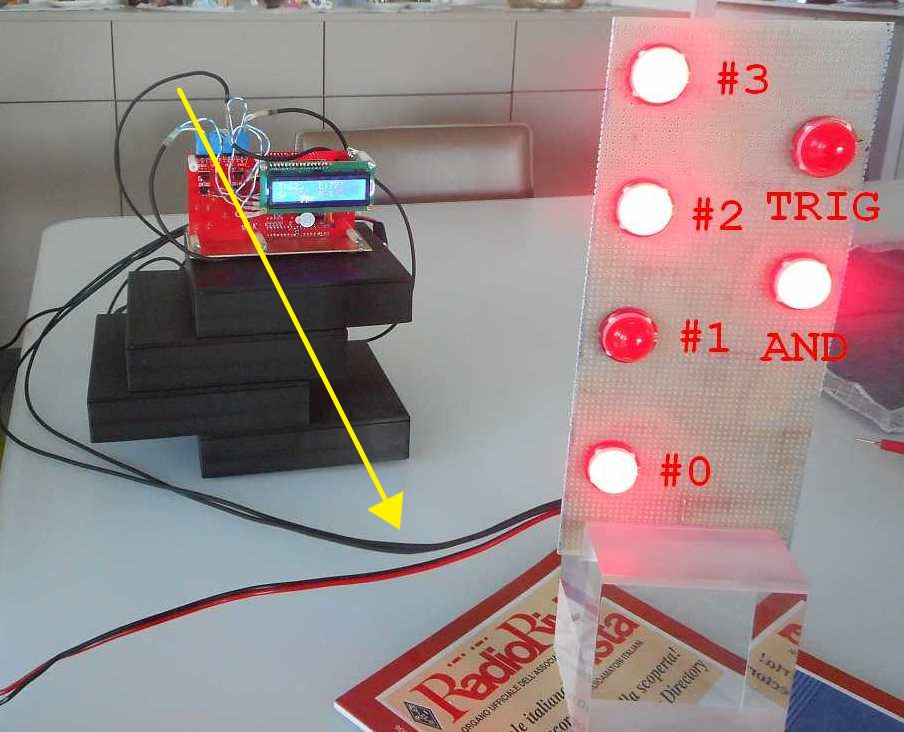
\includegraphics[width=0.35\textwidth]{TRIGGER and(3-0)_event 3-2-0.jpg}
\caption{Test di funzionamento dell'apparato scintillatore.}
\label{Telescopio}

\end{figure}

\subsection{Micromegas}
La micromegas (micro-mesh gaseous structure, MM) è un contatore a valanga a facce piane parallele che consiste in regione di deriva ($\sim 5\,\text{mm}$) e di una moltiplicativa posta tra la micromesh e gli elettrodi di read-out ($\sim 128\,\upmu\text{m} $). 
Quando una particella carica attraversa il detector produce elettroni di ionizzazione nella regione di deriva/conversione, che successivamente si spostano verso la zona moltiplicativa attraverso i buchi nella griglia della mesh, dove vengono amplificati. 

\begin{figure}[!h]
    \centering
    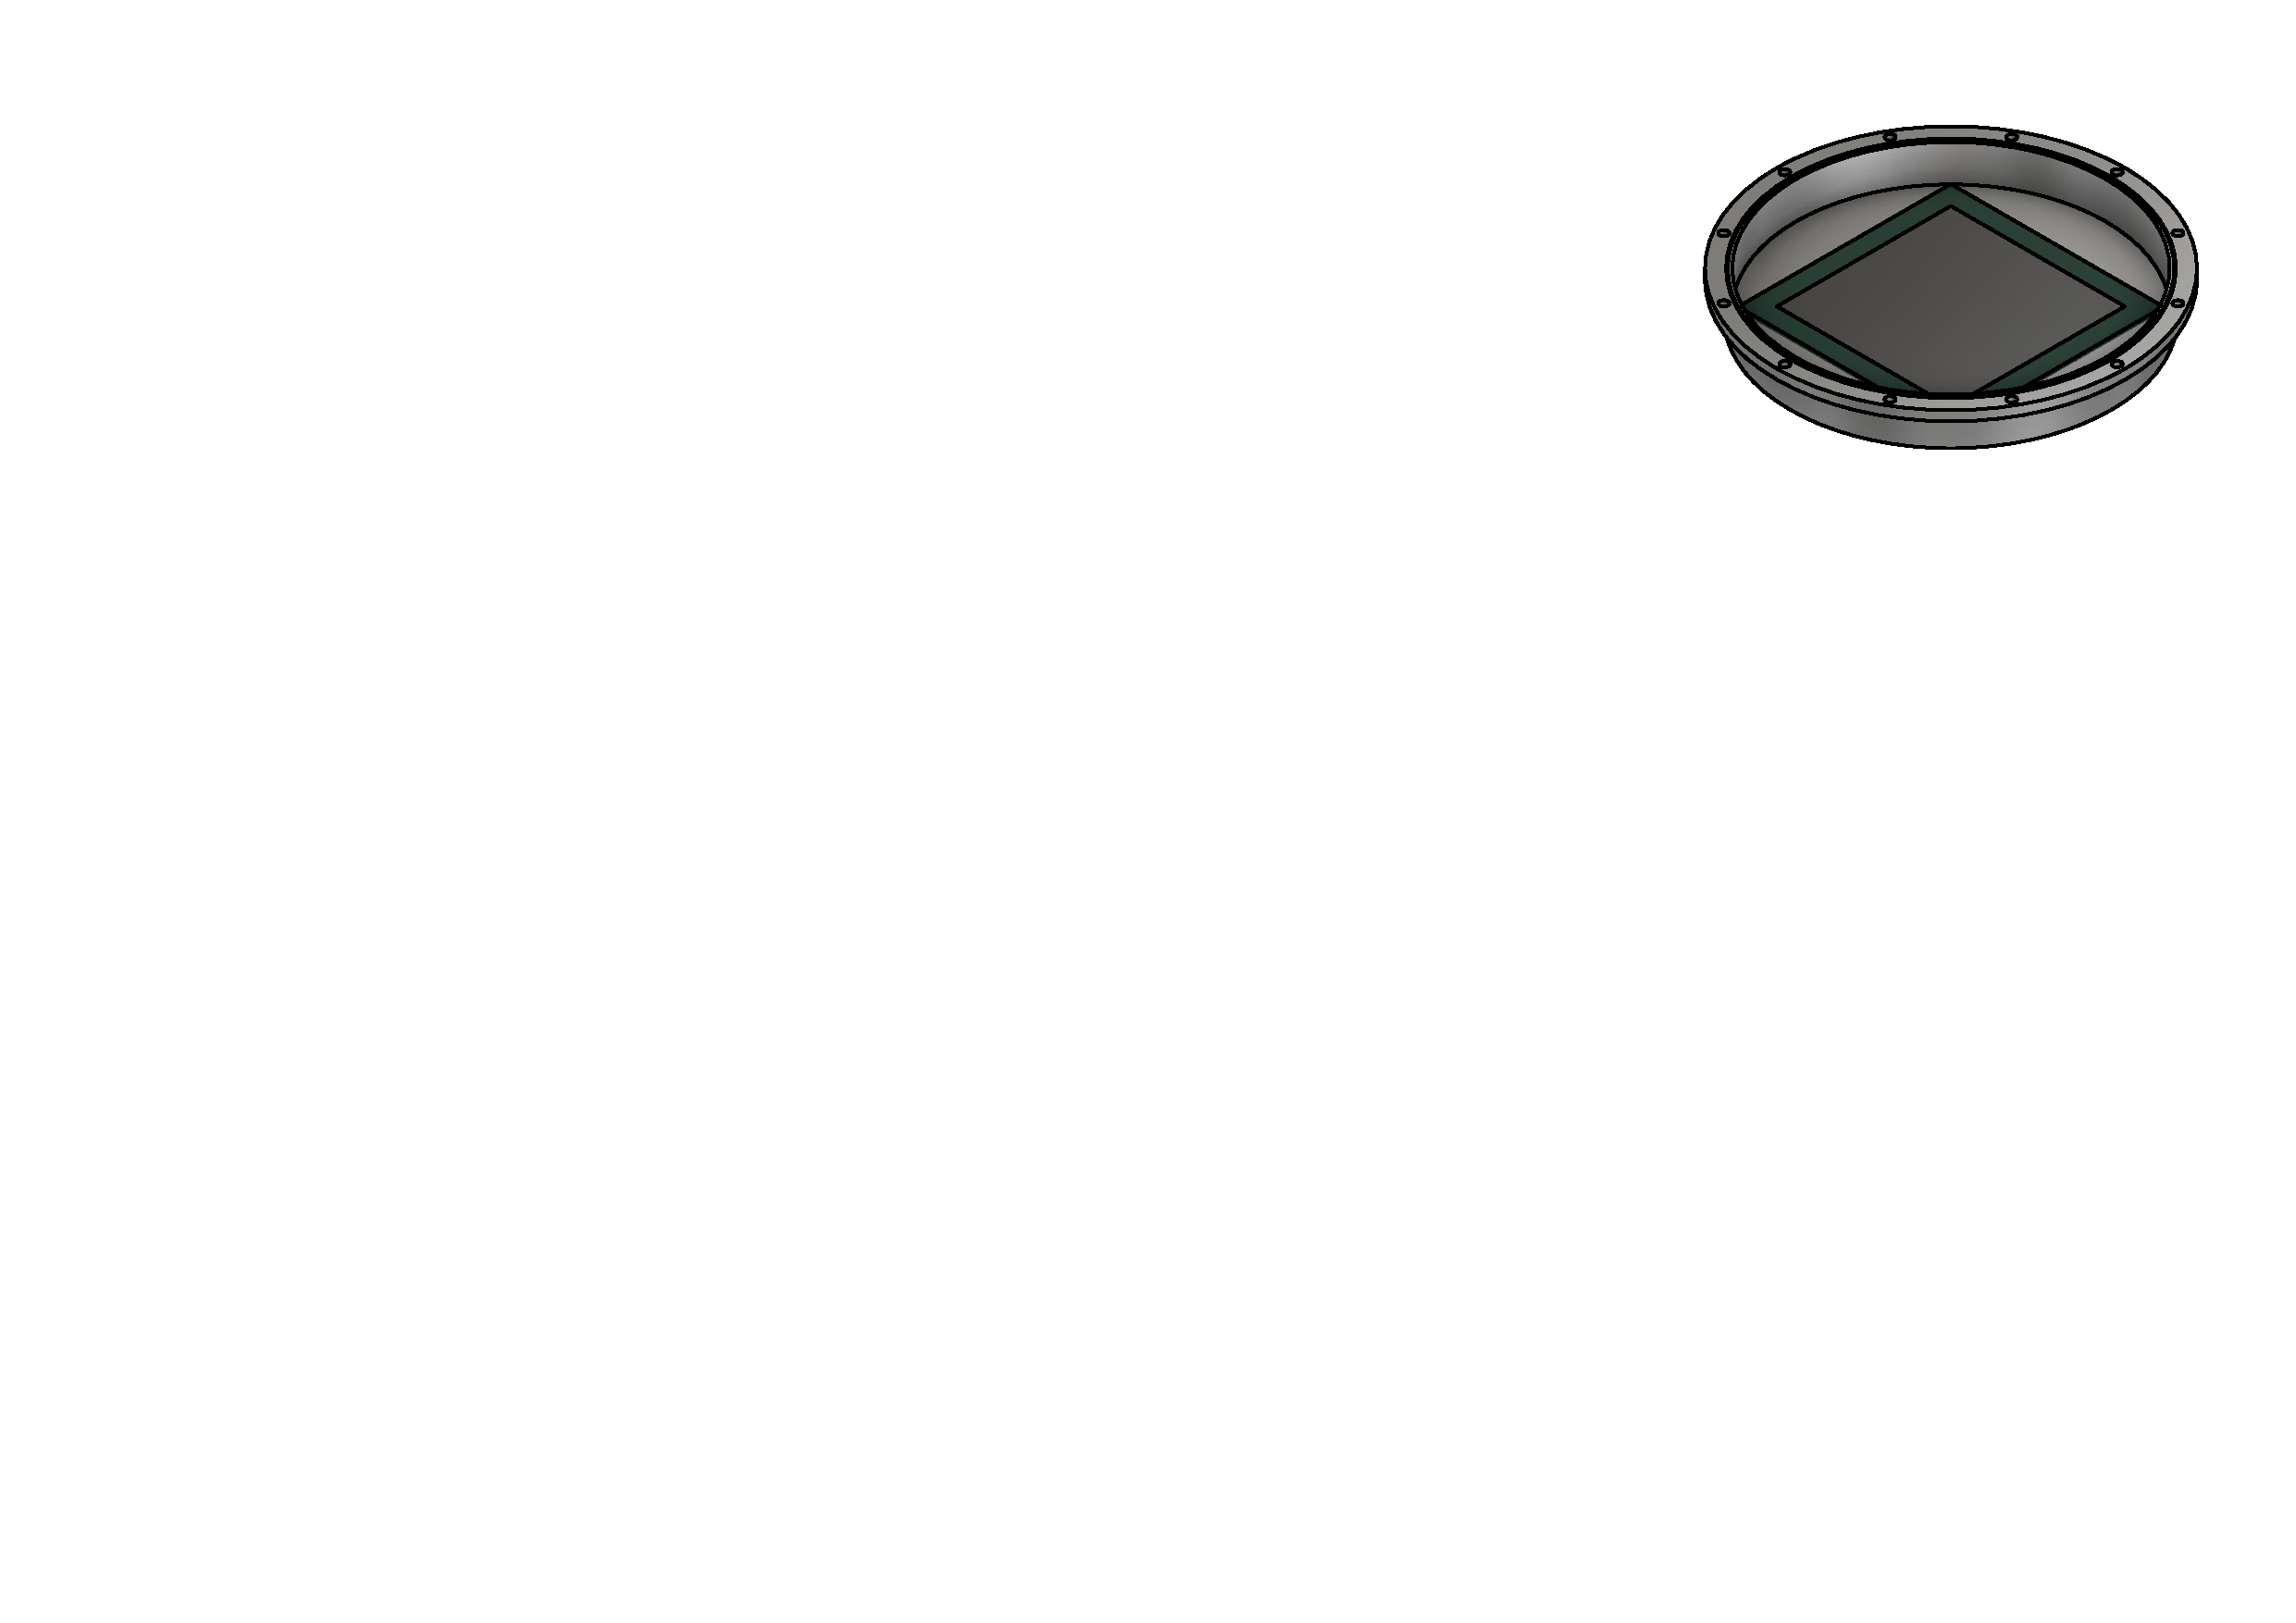
\includegraphics[width=0.4\textwidth]{Micromegas_Disegno.pdf}
    \caption{Proiezione della micromegas e del supporto appositamente progettate per il nostro esperimento.}
    \label{Micromegas_Disegno}
\end{figure}

La micromegas che si implementerà è unica nel suo genere perché ottimizzata anche per la rivelazione degli ENA (atomi neutri di bassa energia) che vengono ionizzati a seguito dell'attraversamento di un foglio di carbonio posto sulla finestra di rivelazione della MM. 
Viste le dimensioni e i pesi non sarà possibile equipaggiarla con un read-out standard, ma sarà letto soltanto il segnale della mesh, corrispondente all’OR di tutte le strip e questo non ci permetterà di fare misure di posizione. Tuttavia, questo tipo di lettura è sufficiente per effettuare misure di flusso e di efficienza della camera stessa. Rispetto ad una micromegas standard, realizzate in dimensioni anche di diversi m$^2$ per i grandi esperimenti del CERN come ATLAS, grande attenzione sarà dedicata nella costruzione della meccanica di supporto con lo scopo di permettere al detector di operare senza un sistema di flussaggio di gas per tutta la durata del volo del pallone. 
 
\begin{figure}
	\centering
    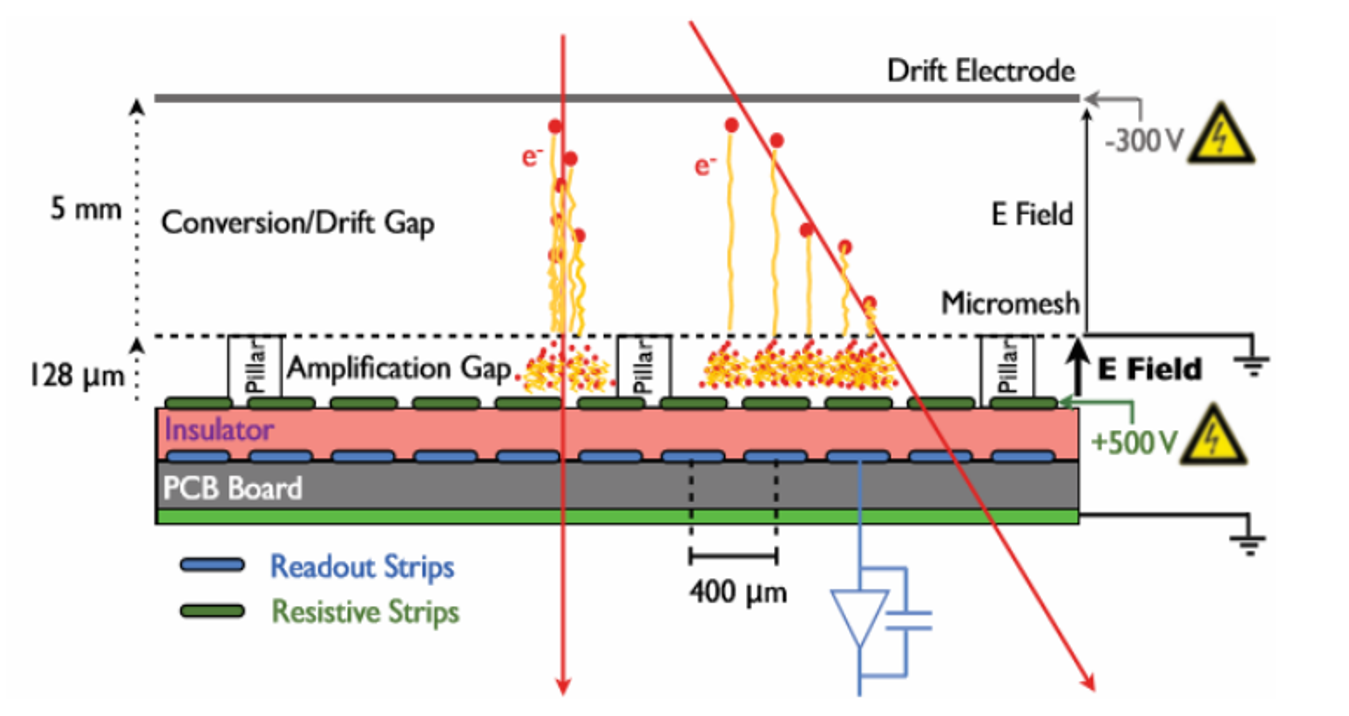
\includegraphics[width=0.4\textwidth]{schema_micromegas.png}
    \caption{Schema concettuale di una "bulk micromegas". Le dimensioni del gap di amplificazione ed i valori di tensione sono ottimizzati per la rivelazione di muoni di alta energia.}
    \label{fisica_micromegas}
\end{figure}

\section{Rivelatore di neutroni}
Essendo particelle neutre, i neutroni non possono essere rivelati con \emph{detectors} che sfruttano il principio della ionizzazione, perciò una strumentazione dedicata è necessaria. I rivelatori di neutroni sono basati sulla rivelazione di prodotti secondari (fotoni, particelle cariche) dalle reazioni nucleari indotte dall'urto del neutrone su elementi tipo $^{10}$B o $^6$Li. Questo sistema di rivelazione è efficace solo per i neutroni termici, e proprio per questo è ideale per la misura sul flusso di neutroni che ci proponiamo di svolgere. Entrambi i sistemi che vengono proposti sono basati su una plastica drogata accoppiata ad un rivelatore di fotoni: i costi ed il peso sono simili, ma hanno pregi e difetti che richiedono un approfondimento maggiore per scegliere quale utilizzare nell'esperienza (\emph{che svolgeremo appena il progetto venga approvato}). 

\subsection{Prima proposta}
Un sistema utilizza come rivelatore il dosimetro CT007-T della GammaGuard. Il dosimetro comunica tramite Bluetooth con una applicazione per Android, dove i dati (compresi data e coordinate GPS) vengono conservati. Il salvataggio dei dati su un file .csv viene eseguito attraverso comandi manuali alla fine dell'acquisizione, perciò questo sistema prevede la necessità di un cellulare che rimanga funzionante in volo e dopo l'atterraggio. Un cellulare che soddisfa le richieste è il Blackview BV4900 ProRugged (operatività garantita a temperature nel range [-55, +70] °C). 

\textbf{Pregi}: 1) un rivelatore pronto all'uso e con una interfaccia semplice e dai risultati garantiti; 2) il peso complessivo (400 g); 3) l'alimentazione autonoma (due pile AA per il dosimetro, la batteria per il cellulare); 4) il cellulare supporta la ricarica inversa, perciò potrebbe essere utilizzato come power bank (\emph{da valutare in laboratorio}). 

\textbf{Difetti}: 1) Impossibilità di salvare i dati automaticamente. 

\subsection{Seconda proposta}
La seconda proposta prevede di utilizzare un rivelatore della ditta Scionix che accoppia un rivelatore di fotoni a semiconduttore a un materiale drogato con $^6$Li. Il sistema viene letto da un circuito elettronico simile a quello già montato per il rivelatore di particelle cariche (e sfrutta parte di quella elettronica).
\textbf{Pregi}: 1) Il dispositivo è realizzato dalla ditta Scionix su misura per il nostro scopo, e sfrutta il \emph{know-how} dell'INFN per realizzare un sistema affidabile, perciò il recupero dei dati è garantito; 2) peso ($\sim$ 400 g).
\textbf{Difetti}: 1)  \`E necessario montare un ulteriore power bank per alimentare il rivelatore; 2) l'assemblamento del sistema è più complesso di quello della prima proposta. 




\subsection*{Frame}

Per la realizzazione dell’esperimento è necessario realizzare una struttura di supporto in cui poter fissare tutte le apparecchiature per le rilevazioni. Le linee guida per il progetto sono state essenzialmente 3: 1) Leggerezza della struttura; 2) Resistenza termica; 3) Facilità di realizzazione. Per soddisfare questi 3 punti si è deciso di realizzare una struttura stampata in 3D; il materiale che più si adatta alle richieste è il PETG, un materiale meccanicamente e termicamente resistente e che inoltre è facilmente stampabile. Da esperimenti eseguiti su questo materiale si è visto che con un trattamento termico (“thermal annealing”) in cui si raggiungono i -40°C, il materiale perde solamente il 2-3\% delle caratteristiche meccaniche. Per quanto riguarda la temperatura massima, 80°C sono la temperatura di transizione vetrosa del materiale, oltre la quale il materiale passa a perdere le proprie caratteristiche di rigidezza ed assume un comportamento gommoso. Dai dati di precedenti voli si è visto che le temperature più alte vengono raggiunte solamente localmente dai compenti elettronici, pertanto anche se si dovessero superare i 70°C non sarebbe un problema per la resistenza strutturale dei supporti. In Figura \ref{frame} è riportato il supporto meccanico assemblato con i rivelatori.

\subsection*{Surriscaldamento e coibentazione}
L'apparato per la rivelazione dei RC è molto sensibile alla temperatura, e in particolare questa ne influenza l'efficienza. Salendo in quota, è noto che la temperatura vari nel range $-56^{\circ} \div 15^{\circ}$. Per minimizzare tale variazione si è deciso di coibentare l'apparato con una struttura in polistirolo.

L'elettronica che si vuole utilizzare può facilmente surriscaldarsi (in particolare la FPGA), e ciò può comportare un effetto non controllabile sulla strumentazione. Per minimizzare questo effetto si è pensato di separare fisicamente l'elettronica dall'apparato rivelatore.
% (uno scatch di questa soluzione è illsutrata in Figura \ref{surriscaldamento}).

%\begin{figure}
%    \centering
%    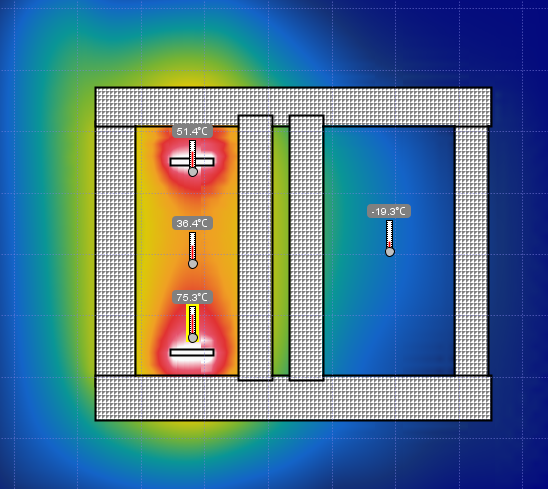
\includegraphics[width=0.3\textwidth]{surriscaldamento.png}
%    \caption{Simulazione \textit{Energy2D}\citep{surriscaldamento}: a sinistra due sorgenti a $80^{\circ}$ con isolamento in polistirolo; a destra uno spazio vuoto in cui allocare l'apparato rivelatore.}
%\end{figure}

Inoltre, la strumentazione stessa potrebbe subire malfunzionamenti a causa dell'elevata temperatura: è in corso una valutazione sulla possibilità di inserire delle strips di rame che permettano di dissipare il calore all'esterno dell'elettronica.

\subsection{Peso e Consumi}
Si è stimato che il peso complessivo della strumentazione (rivelatori+frame+elettronica+alimentazione) è di $\approx 2900\,\text{g}$. Dettagli sul peso di ciascun componente sono riportati in Tabella \ref{tab:lista}. Riguardo il consumo in potenza, è trascurabile per rivelatori, mentre si è stimato che l'elettronica consuma complessivamente $\sim 3.6\,\text{A}$ in 3 ore di volo. Riteniamo che un PowerBank da $7.2\,\text{Ah}$ o maggiore sia sufficiente per alimentare la strumentazione.

\section{Sommario}
\begin{figure}[!hbt]
\centering
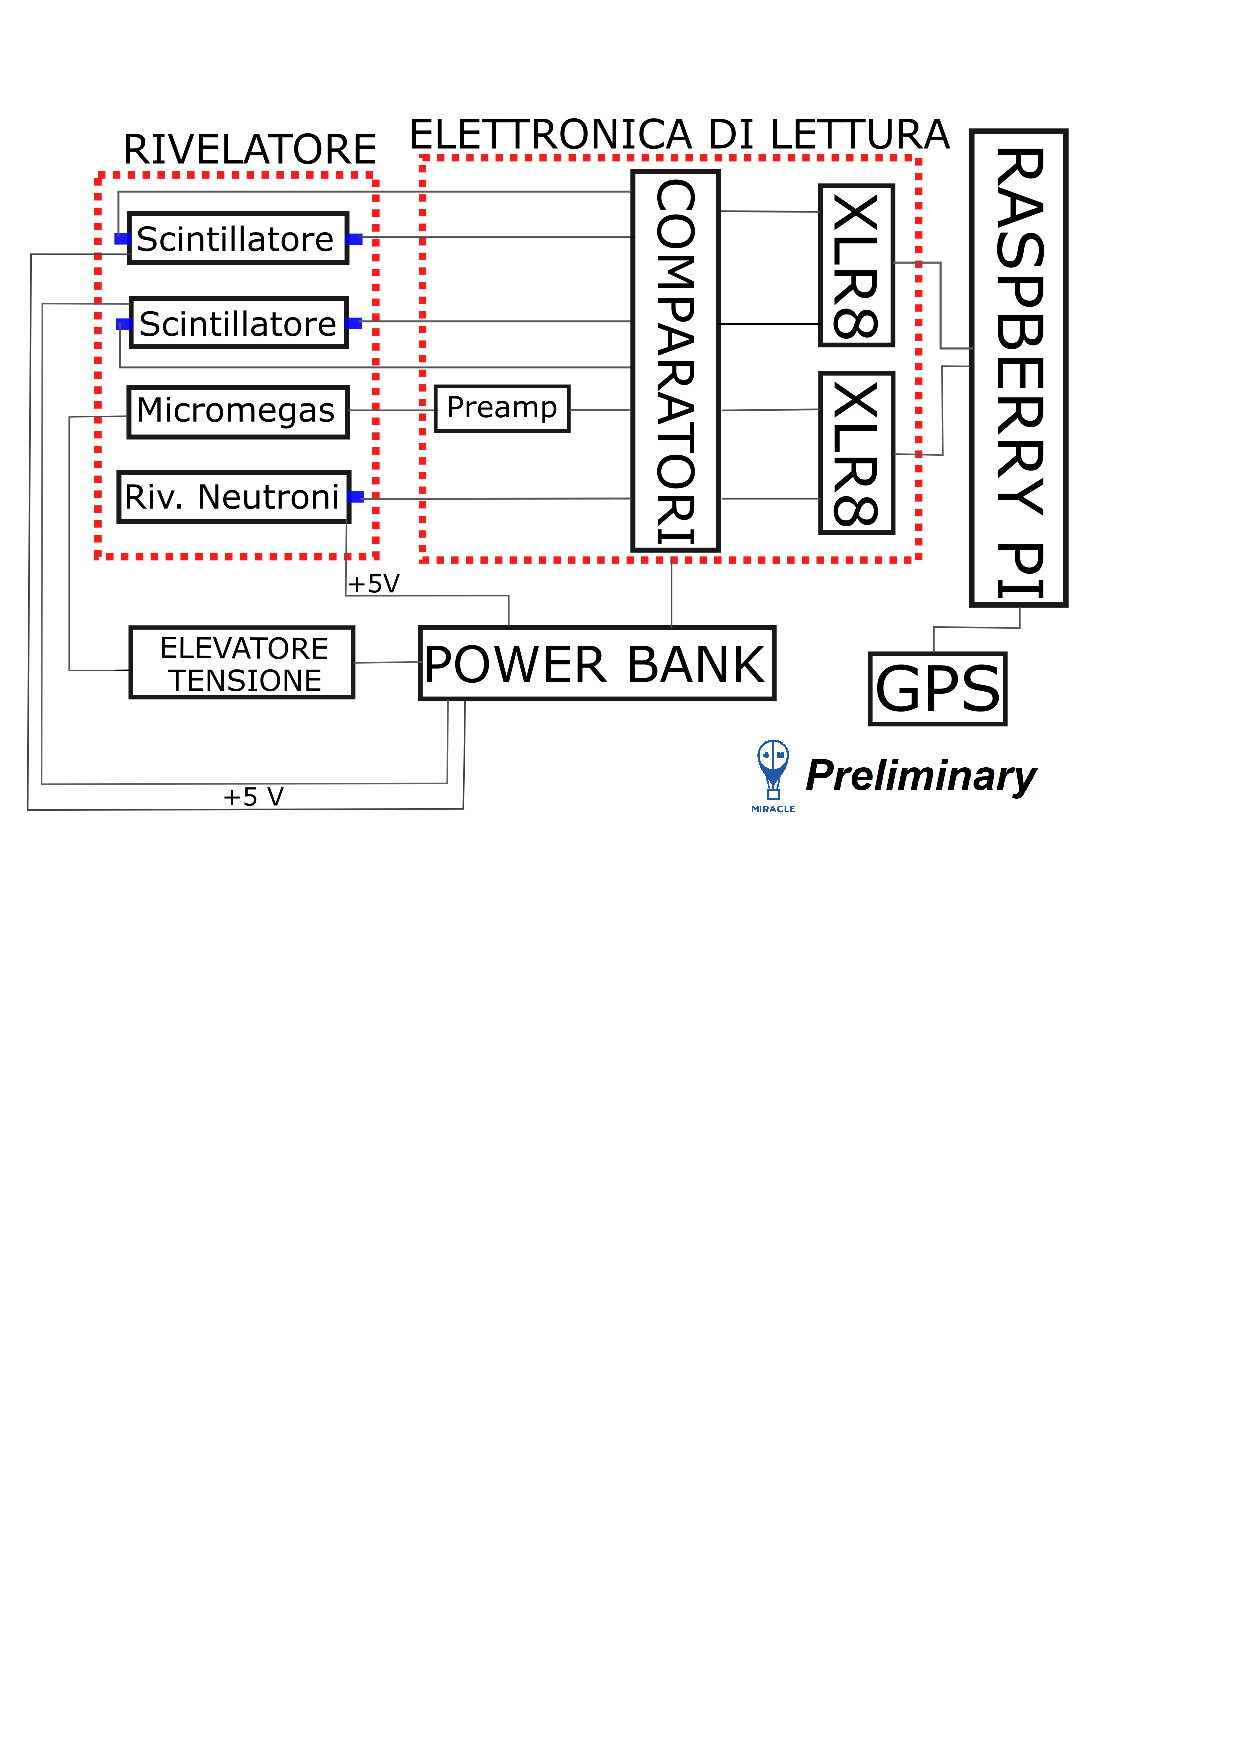
\includegraphics[width=0.5\textwidth]{SCHEMATICA.pdf}
\caption{Schematica riassuntiva dell'apparato rivelatore, dell'elettronica Front-End e dell'elettronica di acquisizioni dati.}
\label{schematica}
\end{figure}
\section*{\begin{large} Ringraziamenti e referenti scientifici \end{large} }
Ringraziamo i ricercatori dell'INFN della sezione di Pisa (Morsani, Paoletti e Pilo) e il Professore G. Lamanna per averci aiutato nello sviluppo della proposta. Il loro interesse e la loro disponibilità (che va ben oltre la strumentazione fornitaci, dandoci la possibilità di fruire di officina, servizio elettronico e laboratori) sono ciò che ci permetterà di \emph{prendere il volo}. 

\newpage

\section{Presentazione del gruppo}

\begin{crewbio}{Adriano Del Vincio}
Laurea triennale in fisica e attualmente iscritto al corso di laurea magistrale in fisica medica. Il mio ruolo all'interno del gruppo è legato all'analisi dati ed ho contribuito a definire la misura proposta del flusso di neutroni in alta atmosfera ed il suo importante legame con la produzione di carbonio 14, impiegato nelle misure di datazione.Inoltre sono stato di supporto a Daniele Passaro nella realizzazione della simulazione dell'interazione di raggi cosmici con l'atmosfera,attraverso l'uso del programma \emph{GEANT4}. 
\end{crewbio}

\begin{crewbio}{Viola Floris}
Laureata in Fisica presso l'Università degli Studi di Perugia. Ho sviluppato una tesi triennale sulla misura dell'energia in Fisica delle Particelle mediante calorimetri, approfondendo l'esperimento NA62 al SPS (Cern). Attenta ai dettagli ed amante delle sfide, mi sono appassionata agli aspetti più sperimentali della fisica delle particelle visitando i tunnel del Cern. Attualmente frequento il Corso di Laurea Magistrale in \emph{Interazioni Fondamentali} all'Università di Pisa, dove, grazie al corso di laboratorio, sto portando avanti misure sui raggi cosmici, sul decadimento del muone e sull'annichilazione del positrone. Do il mio contributo al progetto con l'esperienza acquisita proprio in queste misure.
\end{crewbio}

\begin{crewbio}{Daniele Passaro}
Sono uno studente iscritto al corso di laurea magistrale in Fisica presso l'Università di Pisa, curriculum di  "Interazioni Fondamentali". 
Il mio percorso formativo è incentrato sulla fisica delle particelle, in particolare dando grande attenzione ai metodi sperimentali necessari per l'attività di ricerca in fisica delle alte energie. Riguardo l'attività sperimentale, ho acquisito esperienza seguendo un totale di 6 corsi di laboratorio: 5 durante il corso di laurea triennale in Fisica presso UniSa, incentrati su analisi dati, elettronica digitale e analogica, microelettronica, magnetismo e simulazioni numeriche; uno durante il corso di laurea magistrale, dedicato alla fisica delle interazioni fondamentali ed in particolare sui raggi cosmici.

Nel progetto mi occupo delle simulazioni Monte Carlo, realizzate tramite il toolkit di simulazione avanzata GEANT4 (\textcopyright CERN), e collaboro alla caratterizzazione generale della strumentazione . 
\end{crewbio}

\begin{crewbio}{Domenico Riccardi}
Sono iscritto al corso di laurea magistrale in Fisica presso l'Università di Pisa, curriculum di "Interazioni Fondamentali". I miei interessi sono rivolti, principalmente, alla fisica sperimentale delle alte energie e all'analisi dei dati. L'attività sperimentale svolta nel corso della laurea triennale, frequentando tre laboratori, e in quella magistrale, con il laboratorio d'interazioni fondamentali, mi hanno permesso di approfondire aspetti e problematiche nell'ambito della realizzazione e dell'analisi dei risultati di esperimenti scientifici. La mia passione per la fisica delle alte energie, mi ha portato ad un lavoro di tesi triennale incentrato sullo studio dell'efficienza di ricostruzione dei muoni nel decadimento del mesone $B_c^+$ su simulazioni Monte Carlo prodotte dall'esperimento CMS ad LHC. Nell'esperimento concepito mi occupo dello studio dell'efficienza dell'apparato, che è una variabile fondamentale per le misure di flusso che si vogliono ricavare, e più in generale sulla sua caratterizzazione.
\end{crewbio}

\begin{crewbio}{Marco Riggirello}
Sono uno studente magistrale del dipartimento di Fisica dell'Università di Pisa iscritto al curriculum di \emph{Fisica delle Interazioni Fondamentali}. Per la laurea triennale, conseguita nel 2020, ho presentato una tesi sulla misura della violazione dell'universalità leptonica con l'esperimento CMS in cui ho effettuato un'analisi volta a ottimizzare la precisione della misura di $R(J/\psi)$. Sono molto interessato alle sfide sperimentali della fisica delle alte energie: durante il mio percorso triennale ho seguito numerosi corsi su argomenti di elettronica e analisi dati che sto approfondendo nella prosecuzione magistrale. 

Per il nostro progetto mi sono occupato del \emph{design} dell'apparato e, se sarà effettuato il lancio, contribuir\`o all'analisi dei dati raccolti.
\end{crewbio}

\begin{crewbio}{Antoine Venturini}
Sono uno studente della laurea magistrale in Fisica presso l'Università di Pisa, iscritto al curriculum di Interazioni Fondamentali. Ho coltivato l'interesse per la fisica delle particelle sin dagli anni della triennale, laureandomi (nel 2020) con una tesi sulla misura del decadimento raro del bosone di Higgs in $\mu^+ \mu^-$ di LHC @CERN, e frequentando poi la stessa estate la Summer School tenuta in Giappone dalla collaborazione per l'esperimento Belle 2.  
Insieme ai corsi teorici seguo numerosi corsi dedicati agli aspetti sperimentali della ricerca in fisica delle alte energie, sia all'analisi dati che alla strumentazione per la rivelazione delle particelle.
Ho alle spalle l'esperienza di quattro corsi di laboratorio, dedicati all'analisi dati e all'elettronica analogica e digitale. In particolare, nell'ultimo anno ho condotto esperienze sulla rivelazione di raggi cosmici per mezzo di rivelatori a scintillazione e fototubi. 

Nell'ambito del nostro progetto, mi occupo del sistema per la rivelazioni dei neutroni e dell'analisi dei dati raccolti (se tutto andrà bene). 
\end{crewbio}




\newpage
%\begin{table*}

\centering

\caption{Tabella riassuntiva con componenti e materiale da acquistare, con costi e peso. I due totali si riferiscono ai due differenti \emph{set-up} per il rivelatore di neutroni. \textbf{Entrambe le soluzioni soddisfano i limiti di spesa e di peso.} }
\label{tab:lista}
\begin{tabular}{c  L{0.3\textwidth}  L{0.2\textwidth}  c }\toprule
 & \textbf{Materiale} & \multicolumn{1}{c}{\textbf{Costo}} [\euro ] & Peso [g] \\ \midrule

\multirow{6}*{\textbf{Rivelatore particelle cariche}} &  Lastra scintillatrice con 2 SiPM $\times$ 2 & Gentile concessione INFN (valore forfettario > 1000 \euro) & 504 ciascuna \\
                                             &   Scheda XLR8  %(\url{https://www.mouser.it/ProductDetail/Alorium/XLR8R22M08V5U0DI?qs=sGAEpiMZZMu3sxpa5v1qrr2AbdgXAiuKpEVgyWy0Qeo\%3D}) 
                                             & \centering 76  & - \\ 
                                             & Componenti per PCB & \centering 50  & - \\
                                             & Cavi USB  (USB mini-B $\rightarrow$ USB-A) $\times$ 2 & \centering 3 & - \\
                                             & GPS: modulo Sparkfun GPS module – Copernicus II DIP (GPS-11-858)  %(\url{https://www.digikey.it/product-detail/it/sparkfunelectronics/GPS-11858/1568-1151-ND/5673737})
                                             & \centering 62 & - \\
                                            & Antenna GPS: GPS Cti GPS\_MOD25+2   %(\url{https://it.rs-online.com/web/p/antenne-gps/6673086/})
                                            & \centering 15 & - \\ \cmidrule{2-4}
 &  & \centering 209 + IVA & 1080 \\ \midrule
 
 \multirow{8}*{\textbf{Micromegas}}                   &  Micromegas+gas+circuito alimentazione  &    Gentile concessione INFN  (valore forfettario >2500 \euro) &   -    \\
                                             &  Ibrido per bias e preamp: CAEN WA1422H400F2 
A1422H400F2 - Charge Preamplifier Module, 400mV/MeV 
gain, Cdet<200pF     &  \centering 180     &  -      \\
                                            & Connettori per vuoto & \centering 50 & - \\
                                            &   Scheda XLR8  %(\url{https://www.mouser.it/ProductDetail/Alorium/XLR8R22M08V5U0DI?qs=sGAEpiMZZMu3sxpa5v1qrr2AbdgXAiuKpEVgyWy0Qeo\%3D}) 
                                             & \centering 76  & - \\ 
                                             & Componenti per PCB & \centering 50  & - \\
                                             & Cavi USB  (USB mini-B $\rightarrow$ USB-A) $\times$ 2 & \centering 3 & - \\
                                             & GPS: modulo Sparkfun GPS module – Copernicus II DIP (GPS-11-858)  %(\url{https://www.digikey.it/product-detail/it/sparkfunelectronics/GPS-11858/1568-1151-ND/5673737})
                                             & \centering 62 & - \\
                                            & Antenna GPS: GPS Cti GPS\_MOD25+2   %(\url{https://it.rs-online.com/web/p/antenne-gps/6673086/})
                                            & \centering 15 & - \\ \cmidrule{2-4}
    &   &   \centering 436 + IVA & 900 \\ \midrule
 
\multirow{2}*{\textbf{Rivelatore per neutroni I}}         & CT007-T Thermal Neutron Detector & \centering 850 ca. & 140 \\
                                                & Blackview BV4900 Pro Rugged Smartphone (2020) & \centering 140 & 260 \\ \cmidrule{2-4}
    & & \centering 890 ca. (di cui 140 IVA inclusa) & 400 \\ \cmidrule{1-4}
\textbf{Rivelatore per  neutroni II}    & Rivelatore Scionix & \centering 1095 & - \\
                                            & Componenti per PCB & \centering 50 & - \\ \cmidrule{2-4}
                                    &   &   \centering 1145 + IVA & 400 ca. \\ \midrule
                                    
\textbf{Frame di supporto} & Plastica per la stampa in 3D & \centering 50 & 300 ca. \\ \midrule
\textbf{Alimentatori} & Power Bank Ansmann 10 Ah, 5V, 3 porte USB & \centering 50 ca. & 220 \\ \midrule

&\textbf{TOTALE} & \textbf{1635 \ 1885 + IVA} & \textbf{2900} \\ \bottomrule 
                                            
                                                


\end{tabular}
\end{table*}



\end{document}

